% Options for packages loaded elsewhere
\PassOptionsToPackage{unicode}{hyperref}
\PassOptionsToPackage{hyphens}{url}
%
\documentclass[
  10pt,
]{article}
\title{Supplementary Material}
\author{}
\date{}

\usepackage{amsmath,amssymb}
\usepackage{lmodern}
\usepackage{setspace}
\usepackage{iftex}
\ifPDFTeX
  \usepackage[T1]{fontenc}
  \usepackage[utf8]{inputenc}
  \usepackage{textcomp} % provide euro and other symbols
\else % if luatex or xetex
  \usepackage{unicode-math}
  \defaultfontfeatures{Scale=MatchLowercase}
  \defaultfontfeatures[\rmfamily]{Ligatures=TeX,Scale=1}
\fi
% Use upquote if available, for straight quotes in verbatim environments
\IfFileExists{upquote.sty}{\usepackage{upquote}}{}
\IfFileExists{microtype.sty}{% use microtype if available
  \usepackage[]{microtype}
  \UseMicrotypeSet[protrusion]{basicmath} % disable protrusion for tt fonts
}{}
\makeatletter
\@ifundefined{KOMAClassName}{% if non-KOMA class
  \IfFileExists{parskip.sty}{%
    \usepackage{parskip}
  }{% else
    \setlength{\parindent}{0pt}
    \setlength{\parskip}{6pt plus 2pt minus 1pt}}
}{% if KOMA class
  \KOMAoptions{parskip=half}}
\makeatother
\usepackage{xcolor}
\IfFileExists{xurl.sty}{\usepackage{xurl}}{} % add URL line breaks if available
\IfFileExists{bookmark.sty}{\usepackage{bookmark}}{\usepackage{hyperref}}
\hypersetup{
  pdftitle={Supplementary Material},
  hidelinks,
  pdfcreator={LaTeX via pandoc}}
\urlstyle{same} % disable monospaced font for URLs
\usepackage[margin=1in]{geometry}
\usepackage{listings}
\newcommand{\passthrough}[1]{#1}
\lstset{defaultdialect=[5.3]Lua}
\lstset{defaultdialect=[x86masm]Assembler}
\usepackage{longtable,booktabs,array}
\usepackage{calc} % for calculating minipage widths
% Correct order of tables after \paragraph or \subparagraph
\usepackage{etoolbox}
\makeatletter
\patchcmd\longtable{\par}{\if@noskipsec\mbox{}\fi\par}{}{}
\makeatother
% Allow footnotes in longtable head/foot
\IfFileExists{footnotehyper.sty}{\usepackage{footnotehyper}}{\usepackage{footnote}}
\makesavenoteenv{longtable}
\usepackage{graphicx}
\makeatletter
\def\maxwidth{\ifdim\Gin@nat@width>\linewidth\linewidth\else\Gin@nat@width\fi}
\def\maxheight{\ifdim\Gin@nat@height>\textheight\textheight\else\Gin@nat@height\fi}
\makeatother
% Scale images if necessary, so that they will not overflow the page
% margins by default, and it is still possible to overwrite the defaults
% using explicit options in \includegraphics[width, height, ...]{}
\setkeys{Gin}{width=\maxwidth,height=\maxheight,keepaspectratio}
% Set default figure placement to htbp
\makeatletter
\def\fps@figure{htbp}
\makeatother
\setlength{\emergencystretch}{3em} % prevent overfull lines
\providecommand{\tightlist}{%
  \setlength{\itemsep}{0pt}\setlength{\parskip}{0pt}}
\setcounter{secnumdepth}{-\maxdimen} % remove section numbering
\usepackage{longtable}
\usepackage{lineno}
\makeatletter
\@ifpackageloaded{subfig}{}{\usepackage{subfig}}
\@ifpackageloaded{caption}{}{\usepackage{caption}}
\captionsetup[subfloat]{margin=0.5em}
\AtBeginDocument{%
\renewcommand*\figurename{Supplementary Figure S}
\renewcommand*\tablename{Supplementary Table S}
}
\AtBeginDocument{%
\renewcommand*\listfigurename{List of Figures}
\renewcommand*\listtablename{List of Tables}
}
\newcounter{pandoccrossref@subfigures@footnote@counter}
\newenvironment{pandoccrossrefsubfigures}{%
\setcounter{pandoccrossref@subfigures@footnote@counter}{0}
\begin{figure}\centering%
\gdef\global@pandoccrossref@subfigures@footnotes{}%
\DeclareRobustCommand{\footnote}[1]{\footnotemark%
\stepcounter{pandoccrossref@subfigures@footnote@counter}%
\ifx\global@pandoccrossref@subfigures@footnotes\empty%
\gdef\global@pandoccrossref@subfigures@footnotes{{##1}}%
\else%
\g@addto@macro\global@pandoccrossref@subfigures@footnotes{, {##1}}%
\fi}}%
{\end{figure}%
\addtocounter{footnote}{-\value{pandoccrossref@subfigures@footnote@counter}}
\@for\f:=\global@pandoccrossref@subfigures@footnotes\do{\stepcounter{footnote}\footnotetext{\f}}%
\gdef\global@pandoccrossref@subfigures@footnotes{}}
\newcommand*\listoflistings\lstlistoflistings
\AtBeginDocument{%
\renewcommand*{\lstlistlistingname}{List of Listings}
}
\makeatother
\ifLuaTeX
  \usepackage{selnolig}  % disable illegal ligatures
\fi

\begin{document}
\maketitle

\setstretch{1.4}
\begin{longtable}{lrrrrr}
\caption{CBSAs with Highly Significant $\Delta_{\tilde{H}}$}
\label{tbl:one_pct_diffs}\\
\toprule
                                        name &  $\tilde{H}_{net}$ &  $\tilde{H}_{euc}$ &  $\Delta_{\tilde{H}}$ &  $\Delta_{pct}$ &  $p$ value \\
\midrule
\endfirsthead
\caption[]{CBSAs with Highly Significant $\Delta_{\tilde{H}}$} \\
\toprule
                                        name &  $\tilde{H}_{net}$ &  $\tilde{H}_{euc}$ &  $\Delta_{\tilde{H}}$ &  $\Delta_{pct}$ &  $p$ value \\
\midrule
\endhead
\midrule
\multicolumn{6}{r}{{Continued on next page}} \\
\midrule
\endfoot

\bottomrule
\endlastfoot
                               Anchorage, AK &              0.135 &              0.092 &                 0.043 &           0.470 &       0.002 \\
        Atlanta-Sandy Springs-Alpharetta, GA &              0.321 &              0.293 &                 0.028 &           0.095 &       0.001 \\
            Austin-Round Rock-Georgetown, TX &              0.174 &              0.152 &                 0.023 &           0.150 &       0.006 \\
               Baltimore-Columbia-Towson, MD &              0.331 &              0.284 &                 0.047 &           0.164 &       0.000 \\
              Boston-Cambridge-Newton, MA-NH &              0.254 &              0.228 &                 0.025 &           0.111 &       0.001 \\
             Bridgeport-Stamford-Norwalk, CT &              0.223 &              0.181 &                 0.042 &           0.235 &       0.001 \\
           Charlotte-Concord-Gastonia, NC-SC &              0.264 &              0.233 &                 0.032 &           0.136 &       0.000 \\
          Chicago-Naperville-Elgin, IL-IN-WI &              0.386 &              0.365 &                 0.021 &           0.057 &       0.000 \\
                        Cincinnati, OH-KY-IN &              0.315 &              0.262 &                 0.054 &           0.205 &       0.000 \\
                        Cleveland-Elyria, OH &              0.412 &              0.380 &                 0.033 &           0.086 &       0.004 \\
                                Columbus, OH &              0.273 &              0.234 &                 0.039 &           0.168 &       0.001 \\
             Dallas-Fort Worth-Arlington, TX &              0.255 &              0.218 &                 0.037 &           0.171 &       0.000 \\
                  Denver-Aurora-Lakewood, CO &              0.197 &              0.176 &                 0.021 &           0.120 &       0.002 \\
                 Detroit-Warren-Dearborn, MI &              0.489 &              0.450 &                 0.038 &           0.085 &       0.000 \\
       Hartford-East Hartford-Middletown, CT &              0.313 &              0.264 &                 0.048 &           0.182 &       0.001 \\
        Houston-The Woodlands-Sugar Land, TX &              0.270 &              0.243 &                 0.028 &           0.114 &       0.000 \\
            Indianapolis-Carmel-Anderson, IN &              0.314 &              0.279 &                 0.034 &           0.123 &       0.008 \\
                          Kansas City, MO-KS &              0.294 &              0.266 &                 0.028 &           0.104 &       0.007 \\
                    Lansing-East Lansing, MI &              0.210 &              0.166 &                 0.044 &           0.268 &       0.003 \\
            Las Vegas-Henderson-Paradise, NV &              0.139 &              0.115 &                 0.023 &           0.202 &       0.000 \\
          Los Angeles-Long Beach-Anaheim, CA &              0.284 &              0.264 &                 0.019 &           0.072 &       0.000 \\
          Louisville/Jefferson County, KY-IN &              0.328 &              0.269 &                 0.060 &           0.222 &       0.000 \\
     Miami-Fort Lauderdale-Pompano Beach, FL &              0.354 &              0.323 &                 0.031 &           0.097 &       0.000 \\
                      Milwaukee-Waukesha, WI &              0.429 &              0.398 &                 0.031 &           0.079 &       0.008 \\
     Minneapolis-St. Paul-Bloomington, MN-WI &              0.209 &              0.177 &                 0.032 &           0.182 &       0.000 \\
                       New Haven-Milford, CT &              0.225 &              0.183 &                 0.042 &           0.230 &       0.001 \\
                    New Orleans-Metairie, LA &              0.260 &              0.227 &                 0.032 &           0.142 &       0.009 \\
       New York-Newark-Jersey City, NY-NJ-PA &              0.299 &              0.280 &                 0.019 &           0.067 &       0.000 \\
                           Oklahoma City, OK &              0.253 &              0.219 &                 0.034 &           0.155 &       0.006 \\
                  Olympia-Lacey-Tumwater, WA &              0.112 &              0.077 &                 0.035 &           0.456 &       0.004 \\
                                  Peoria, IL &              0.351 &              0.288 &                 0.063 &           0.218 &       0.004 \\
 Philadelphia-Camden-Wilmington, PA-NJ-DE-MD &              0.326 &              0.302 &                 0.024 &           0.080 &       0.000 \\
                   Phoenix-Mesa-Chandler, AZ &              0.209 &              0.182 &                 0.027 &           0.149 &       0.000 \\
                              Pittsburgh, PA &              0.280 &              0.225 &                 0.055 &           0.245 &       0.000 \\
         Portland-Vancouver-Hillsboro, OR-WA &              0.118 &              0.095 &                 0.024 &           0.249 &       0.001 \\
                                 Redding, CA &              0.120 &              0.084 &                 0.036 &           0.431 &       0.004 \\
        Riverside-San Bernardino-Ontario, CA &              0.169 &              0.144 &                 0.025 &           0.171 &       0.000 \\
                               Rochester, NY &              0.316 &              0.274 &                 0.042 &           0.152 &       0.003 \\
             Sacramento-Roseville-Folsom, CA &              0.152 &              0.129 &                 0.023 &           0.177 &       0.000 \\
                          Salt Lake City, UT &              0.146 &              0.121 &                 0.026 &           0.212 &       0.007 \\
               San Antonio-New Braunfels, TX &              0.231 &              0.200 &                 0.031 &           0.154 &       0.000 \\
          San Diego-Chula Vista-Carlsbad, CA &              0.204 &              0.184 &                 0.019 &           0.105 &       0.009 \\
          San Francisco-Oakland-Berkeley, CA &              0.167 &              0.154 &                 0.014 &           0.089 &       0.008 \\
                     Santa Rosa-Petaluma, CA &              0.118 &              0.088 &                 0.030 &           0.342 &       0.005 \\
                 Seattle-Tacoma-Bellevue, WA &              0.130 &              0.107 &                 0.023 &           0.217 &       0.000 \\
                             Springfield, MA &              0.312 &              0.256 &                 0.056 &           0.217 &       0.000 \\
                            St. Louis, MO-IL &              0.390 &              0.356 &                 0.034 &           0.095 &       0.005 \\
                                Stockton, CA &              0.132 &              0.104 &                 0.027 &           0.262 &       0.009 \\
                             Tallahassee, FL &              0.196 &              0.146 &                 0.050 &           0.346 &       0.005 \\
         Tampa-St. Petersburg-Clearwater, FL &              0.239 &              0.213 &                 0.026 &           0.124 &       0.002 \\
                                  Toledo, OH &              0.268 &              0.218 &                 0.050 &           0.231 &       0.001 \\
  Virginia Beach-Norfolk-Newport News, VA-NC &              0.206 &              0.161 &                 0.045 &           0.277 &       0.000 \\
Washington-Arlington-Alexandria, DC-VA-MD-WV &              0.240 &              0.220 &                 0.020 &           0.092 &       0.001 \\
                            Worcester, MA-CT &              0.200 &              0.156 &                 0.044 &           0.281 &       0.001 \\
\end{longtable}

\begin{figure}
\hypertarget{fig:nup}{%
\centering
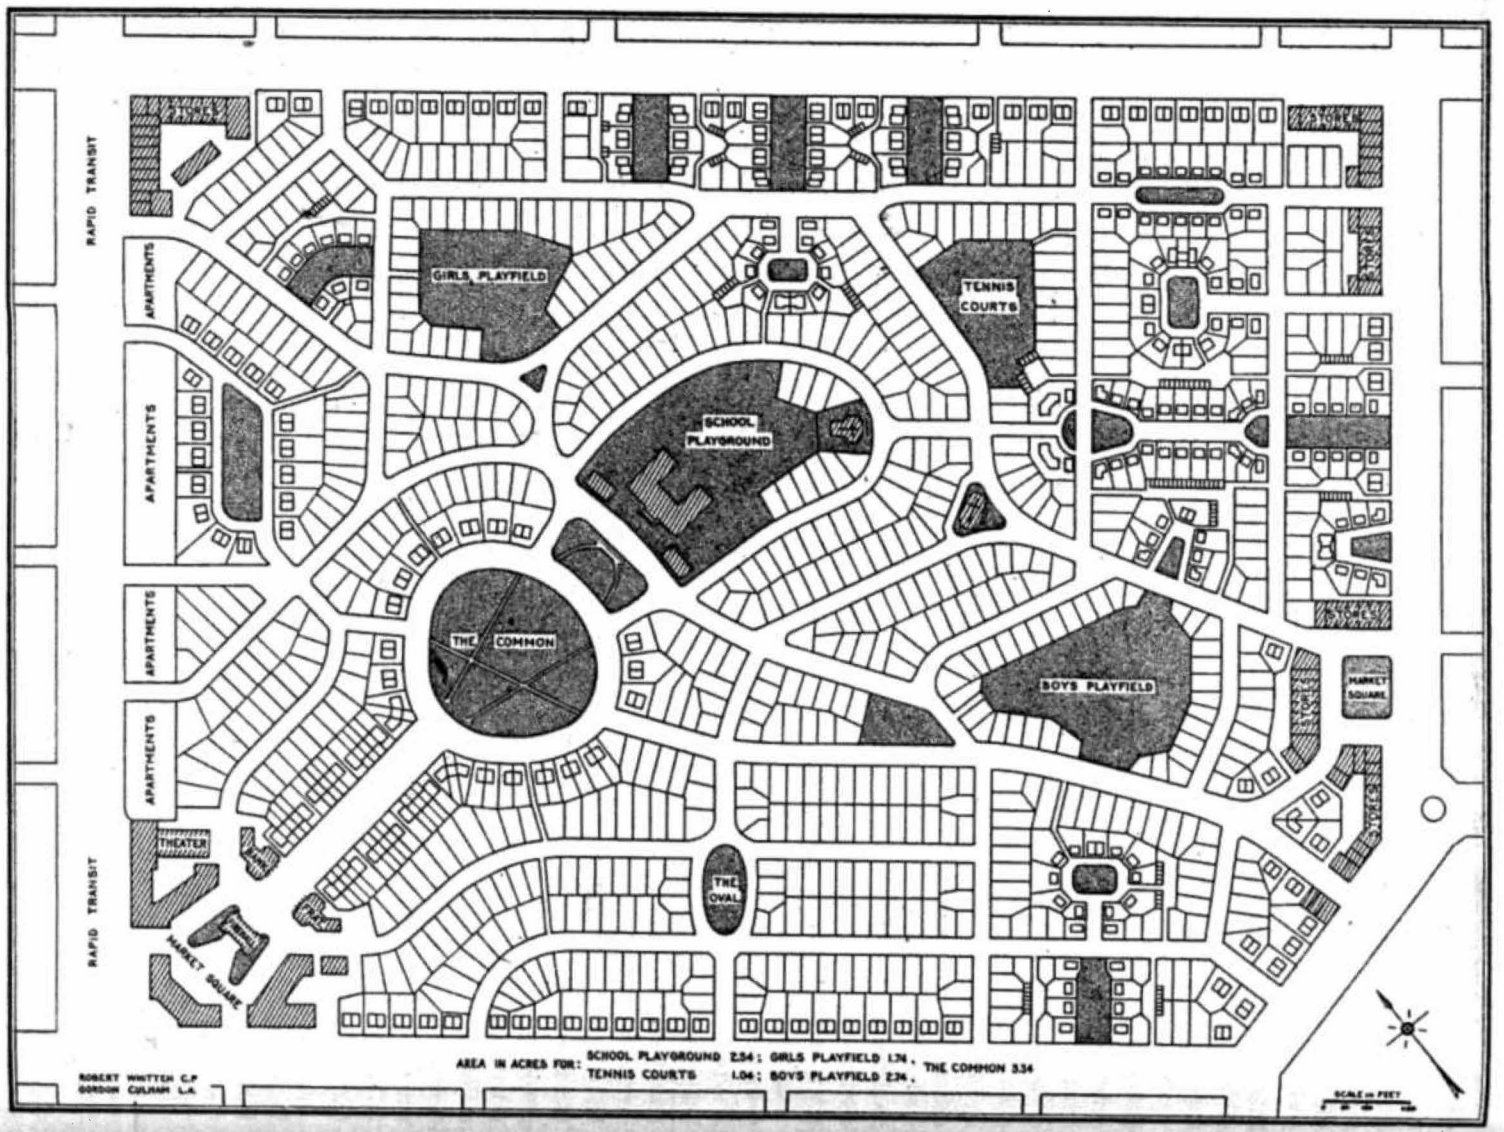
\includegraphics[width=0.85\textwidth,height=\textheight]{./perry_neighborhood_unit.png}
\caption{The ``Neighborhood Unit'' as shown in Perry
(1929)}\label{fig:nup}
}
\end{figure}

\begin{pandoccrossrefsubfigures}

\subfloat[Segregation based on planar and network distances by CBSA. The
45-degree line of equality is shown as
dashed.]{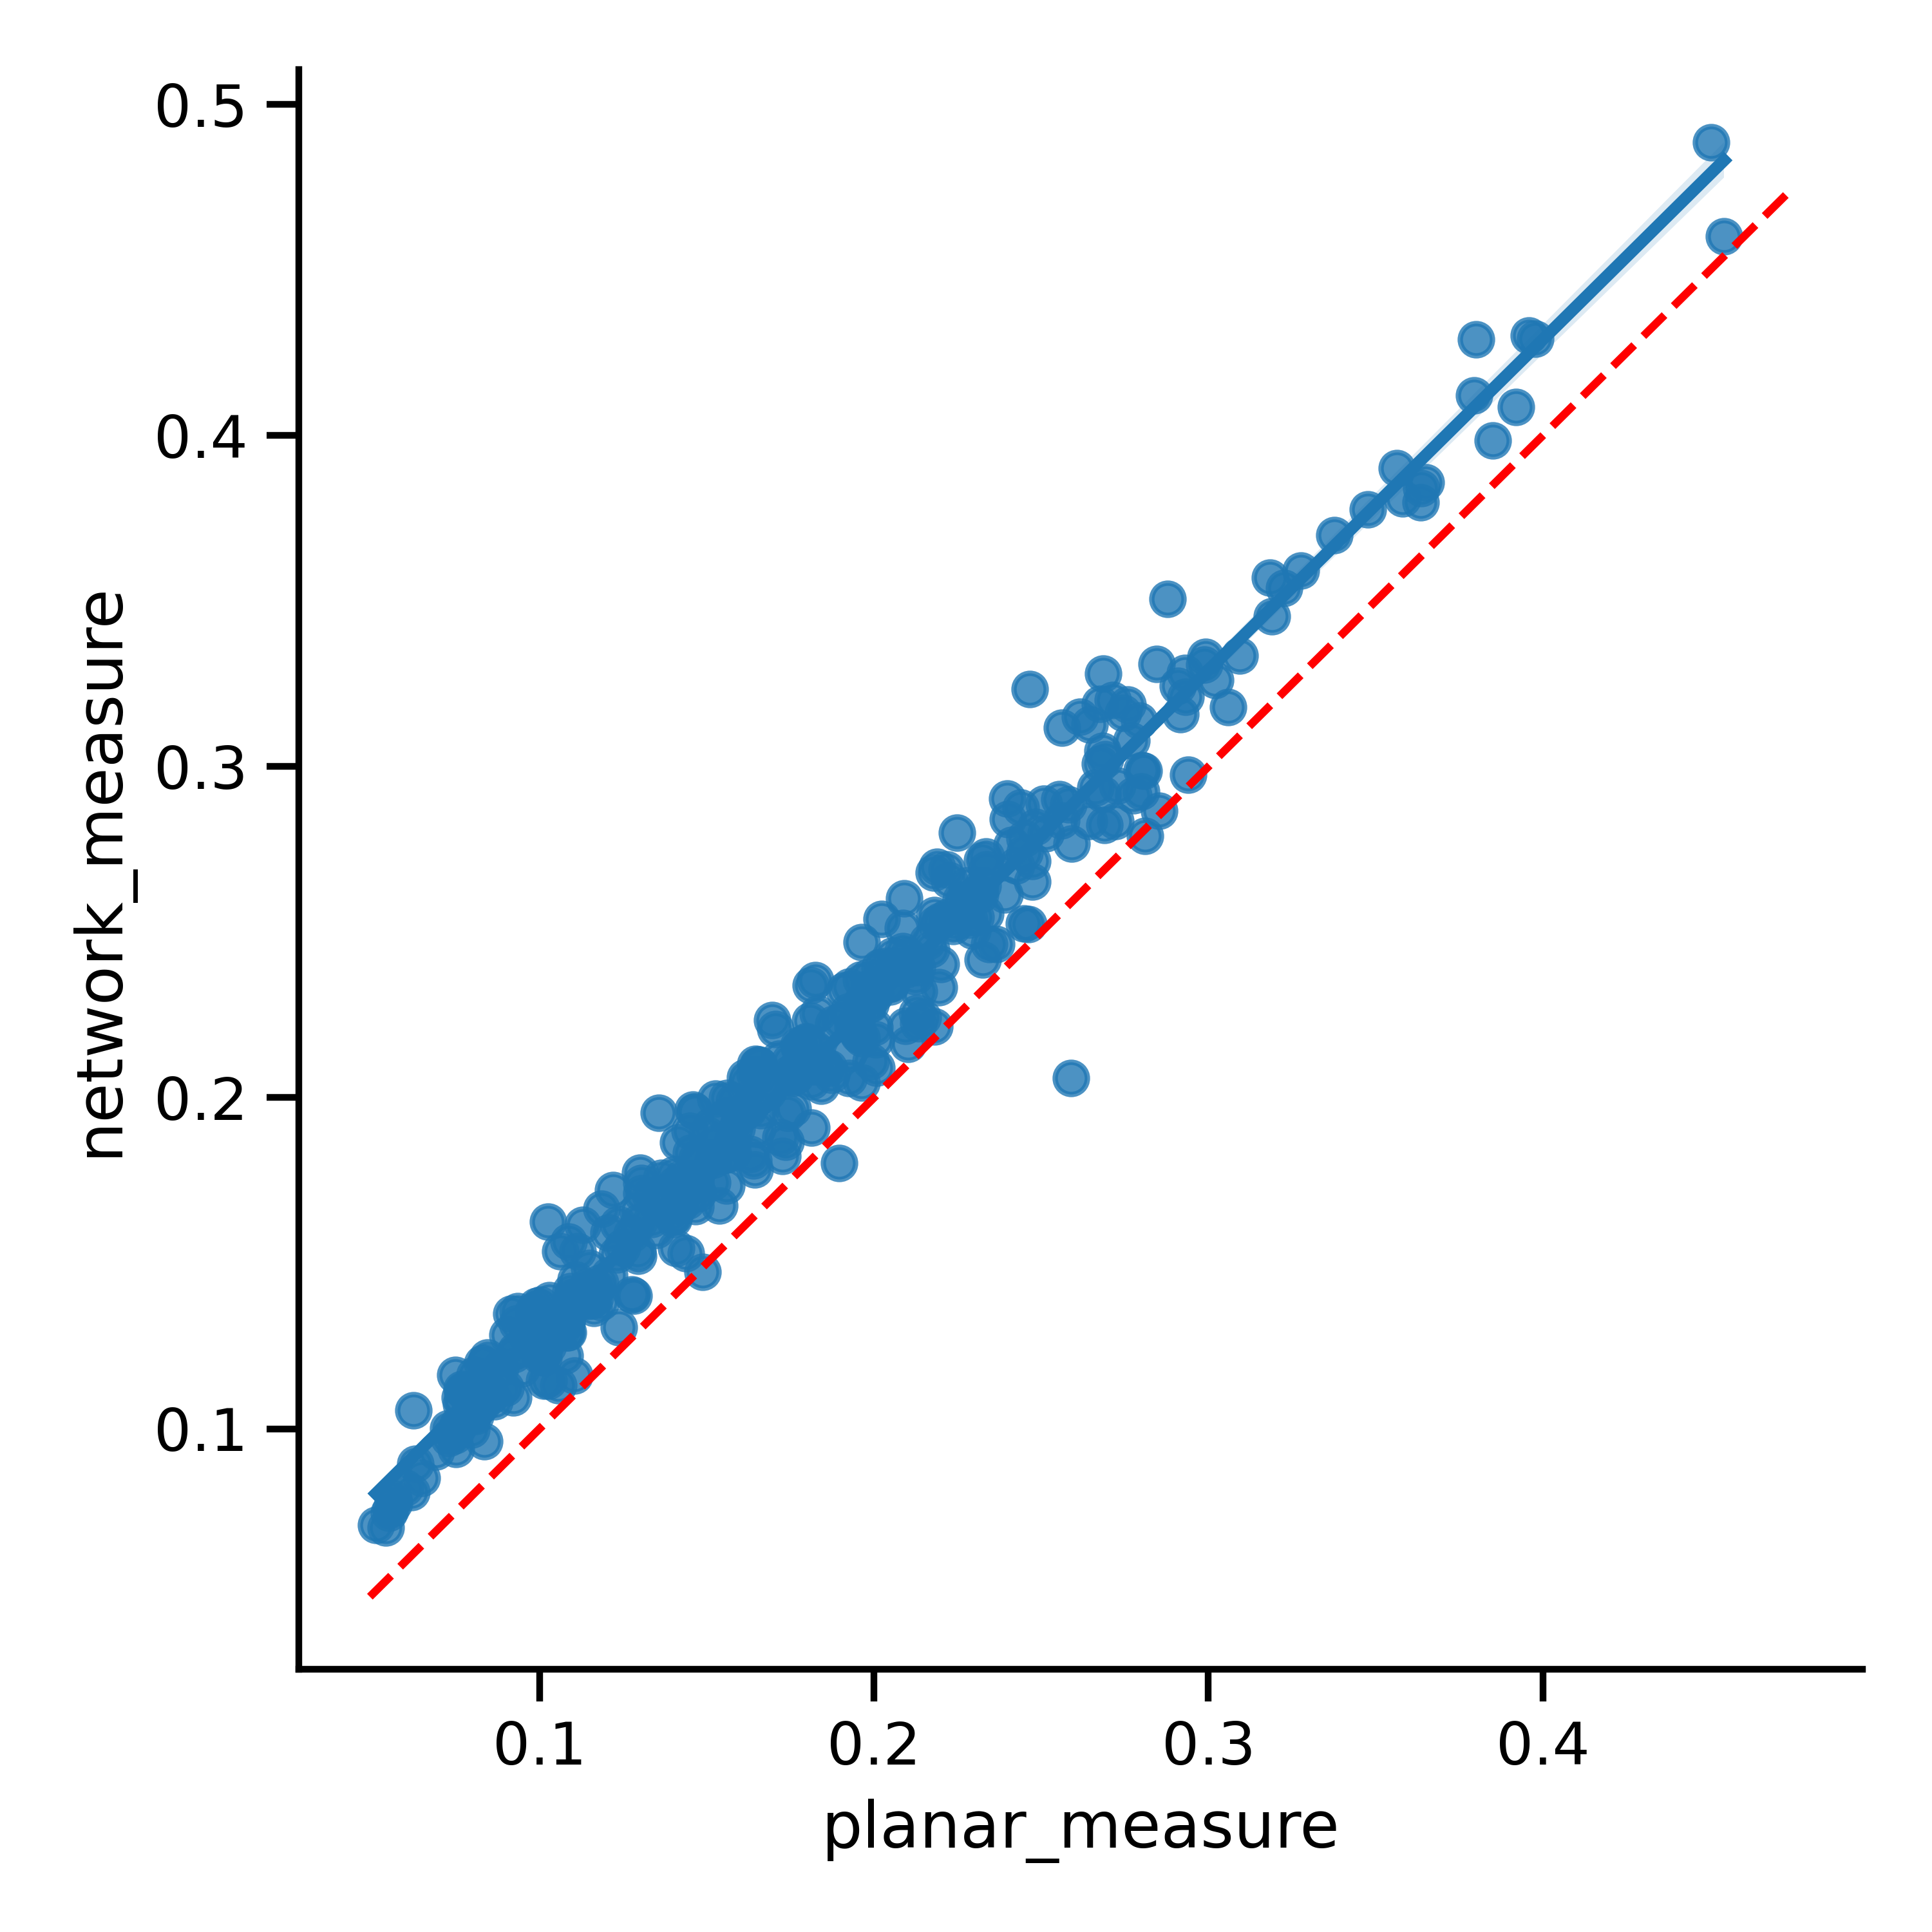
\includegraphics[width=0.45\textwidth,height=\textheight]{./scatter.png}\label{fig:scatter}}
\subfloat[Histogram of \% Differences in Segregation
Measures]{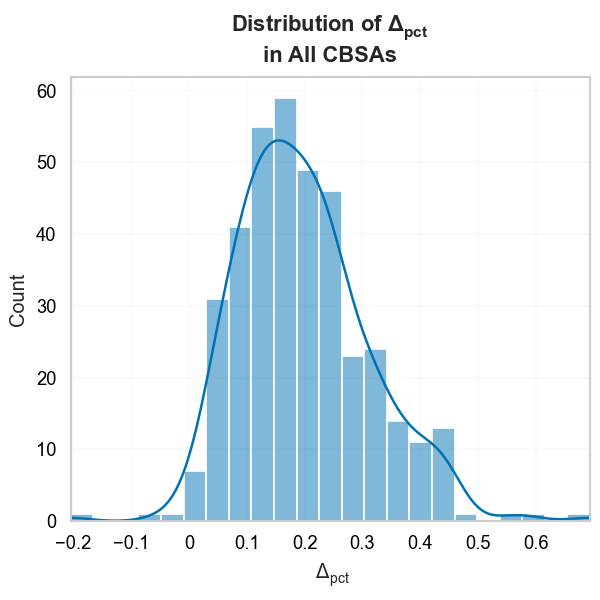
\includegraphics[width=0.45\textwidth,height=\textheight]{./diff_hist.png}\label{fig:diff_hists}}

\caption[{Network vs.~Euclidean-based Segregation Indices}]{Network
vs.~Euclidean-based Segregation Indices}

\label{fig:net_vs_euc}

\end{pandoccrossrefsubfigures}

\begin{figure}
\hypertarget{fig:correlations}{%
\centering
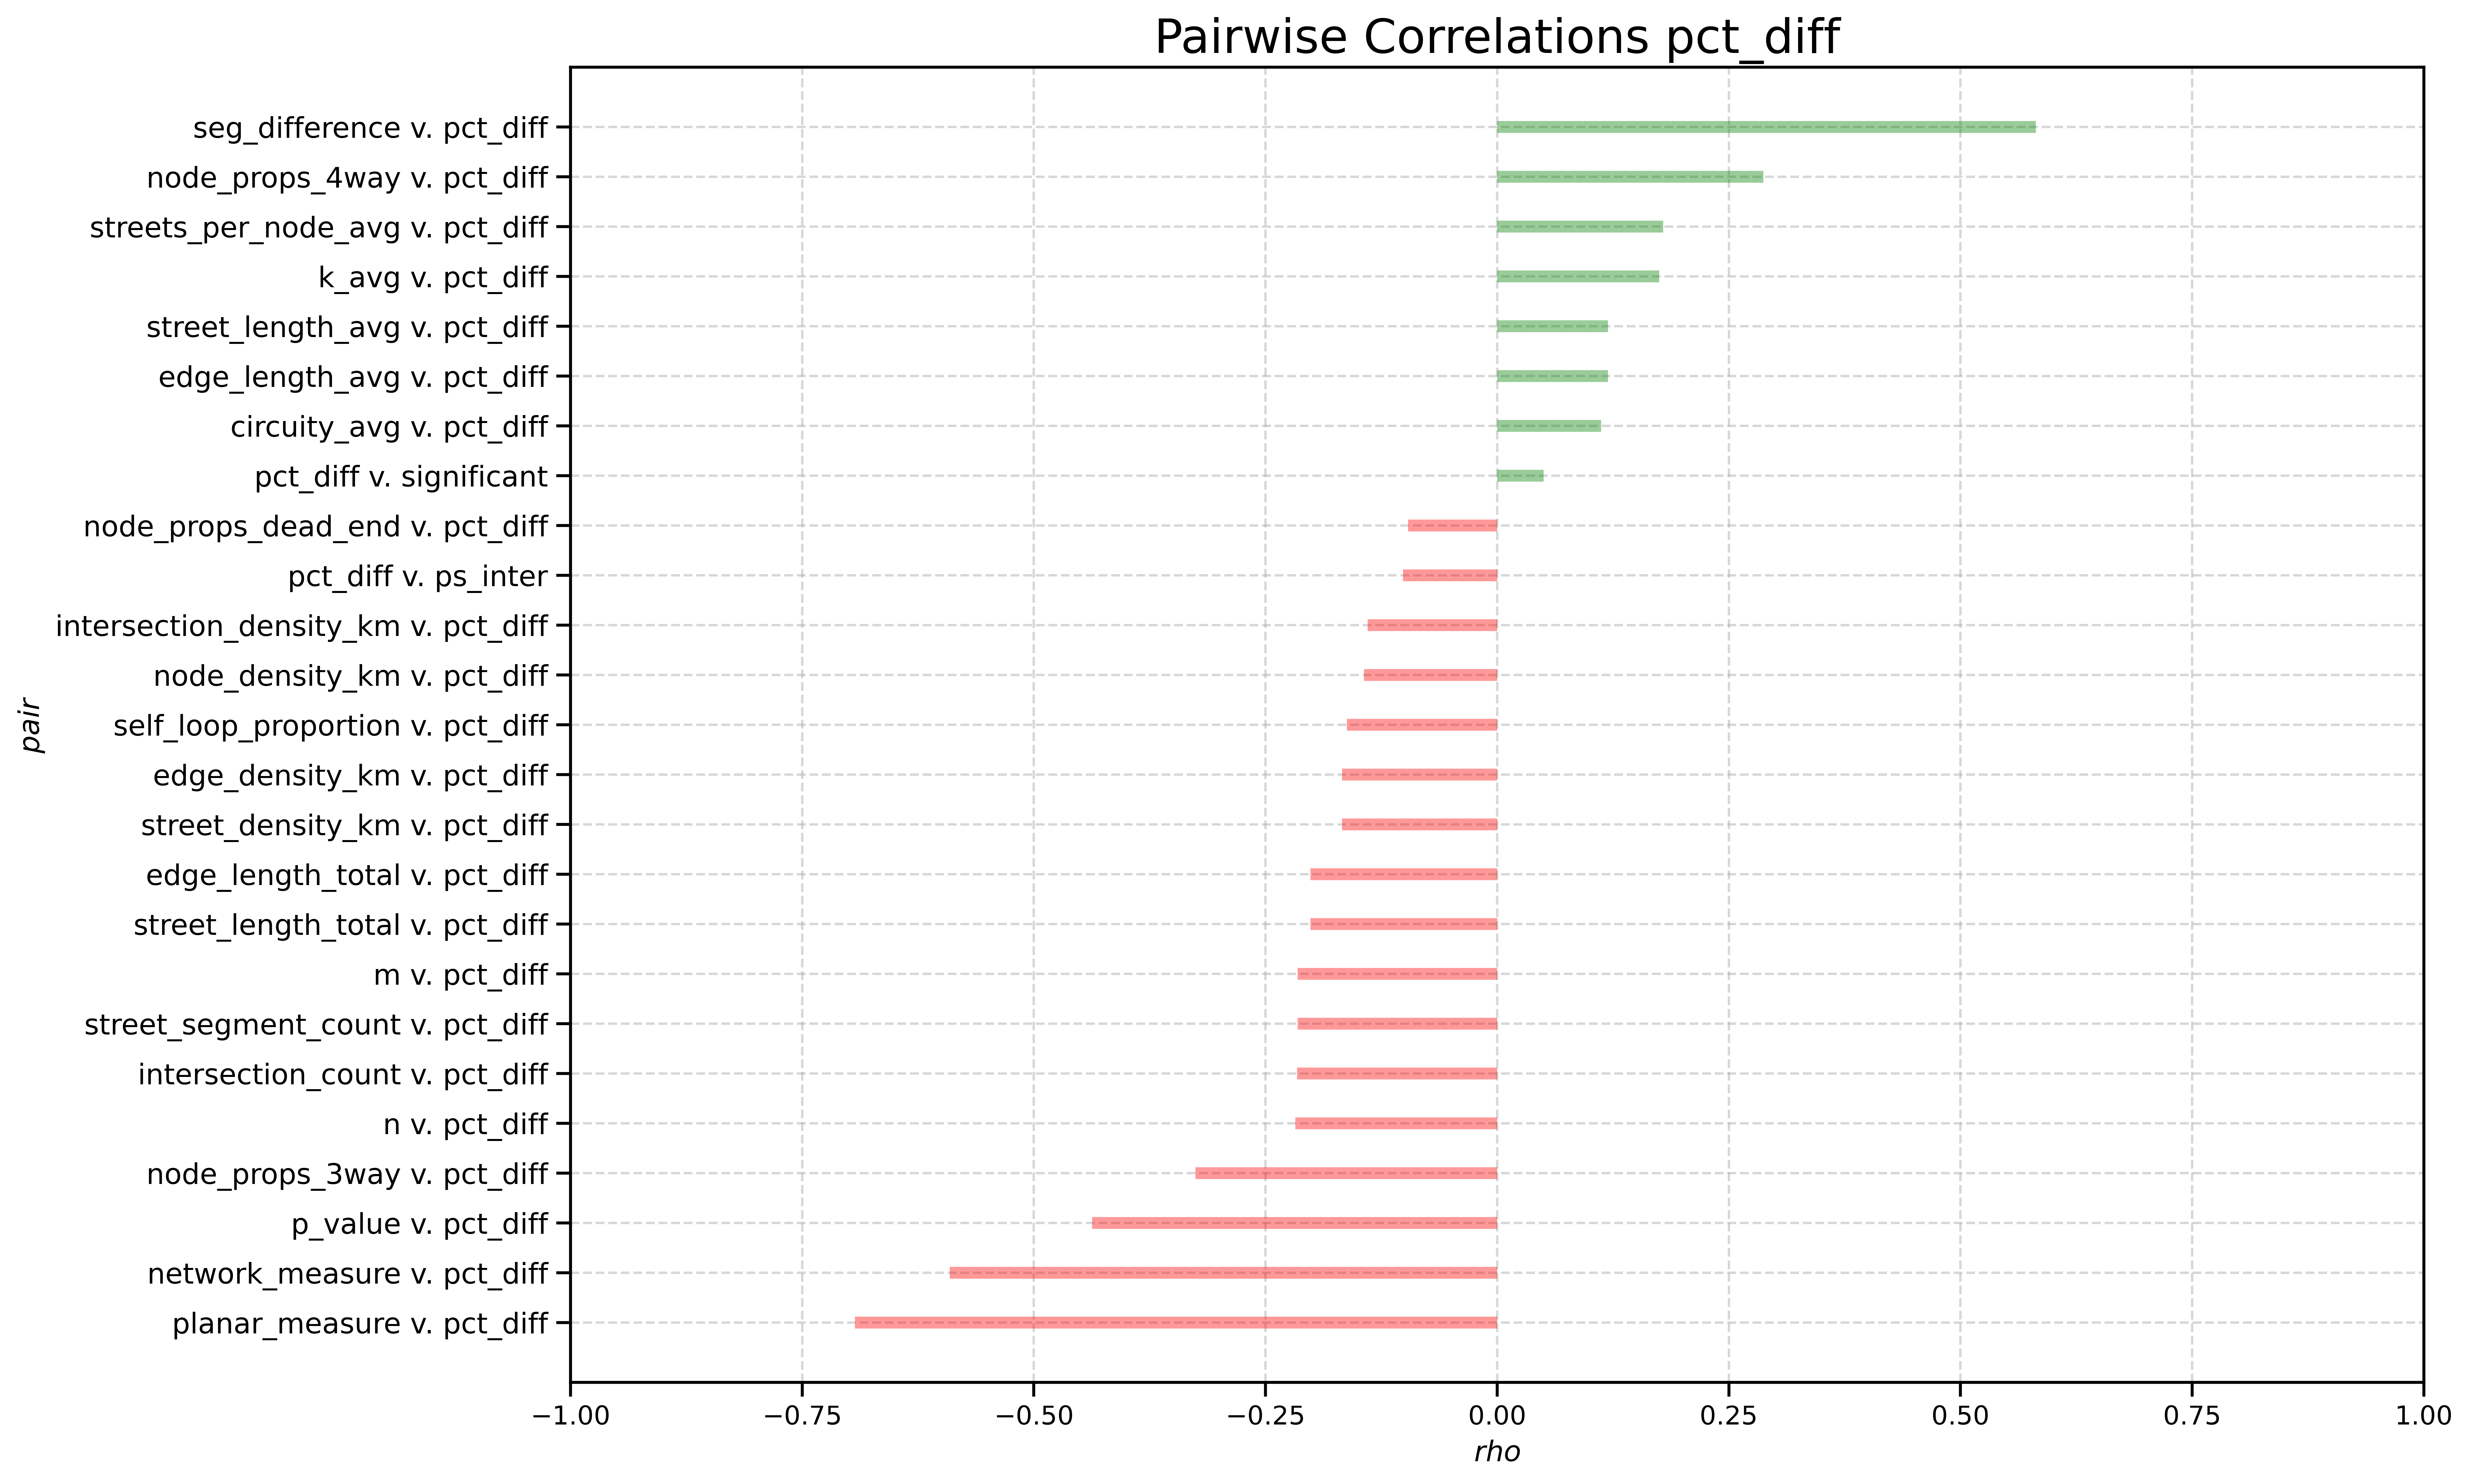
\includegraphics[width=0.9\textwidth,height=\textheight]{./correlations.png}
\caption{Correlates of \(\Delta_{\tilde{H}}\)}\label{fig:correlations}
}
\end{figure}

\begin{figure}
\hypertarget{fig:multiscalar}{%
\centering
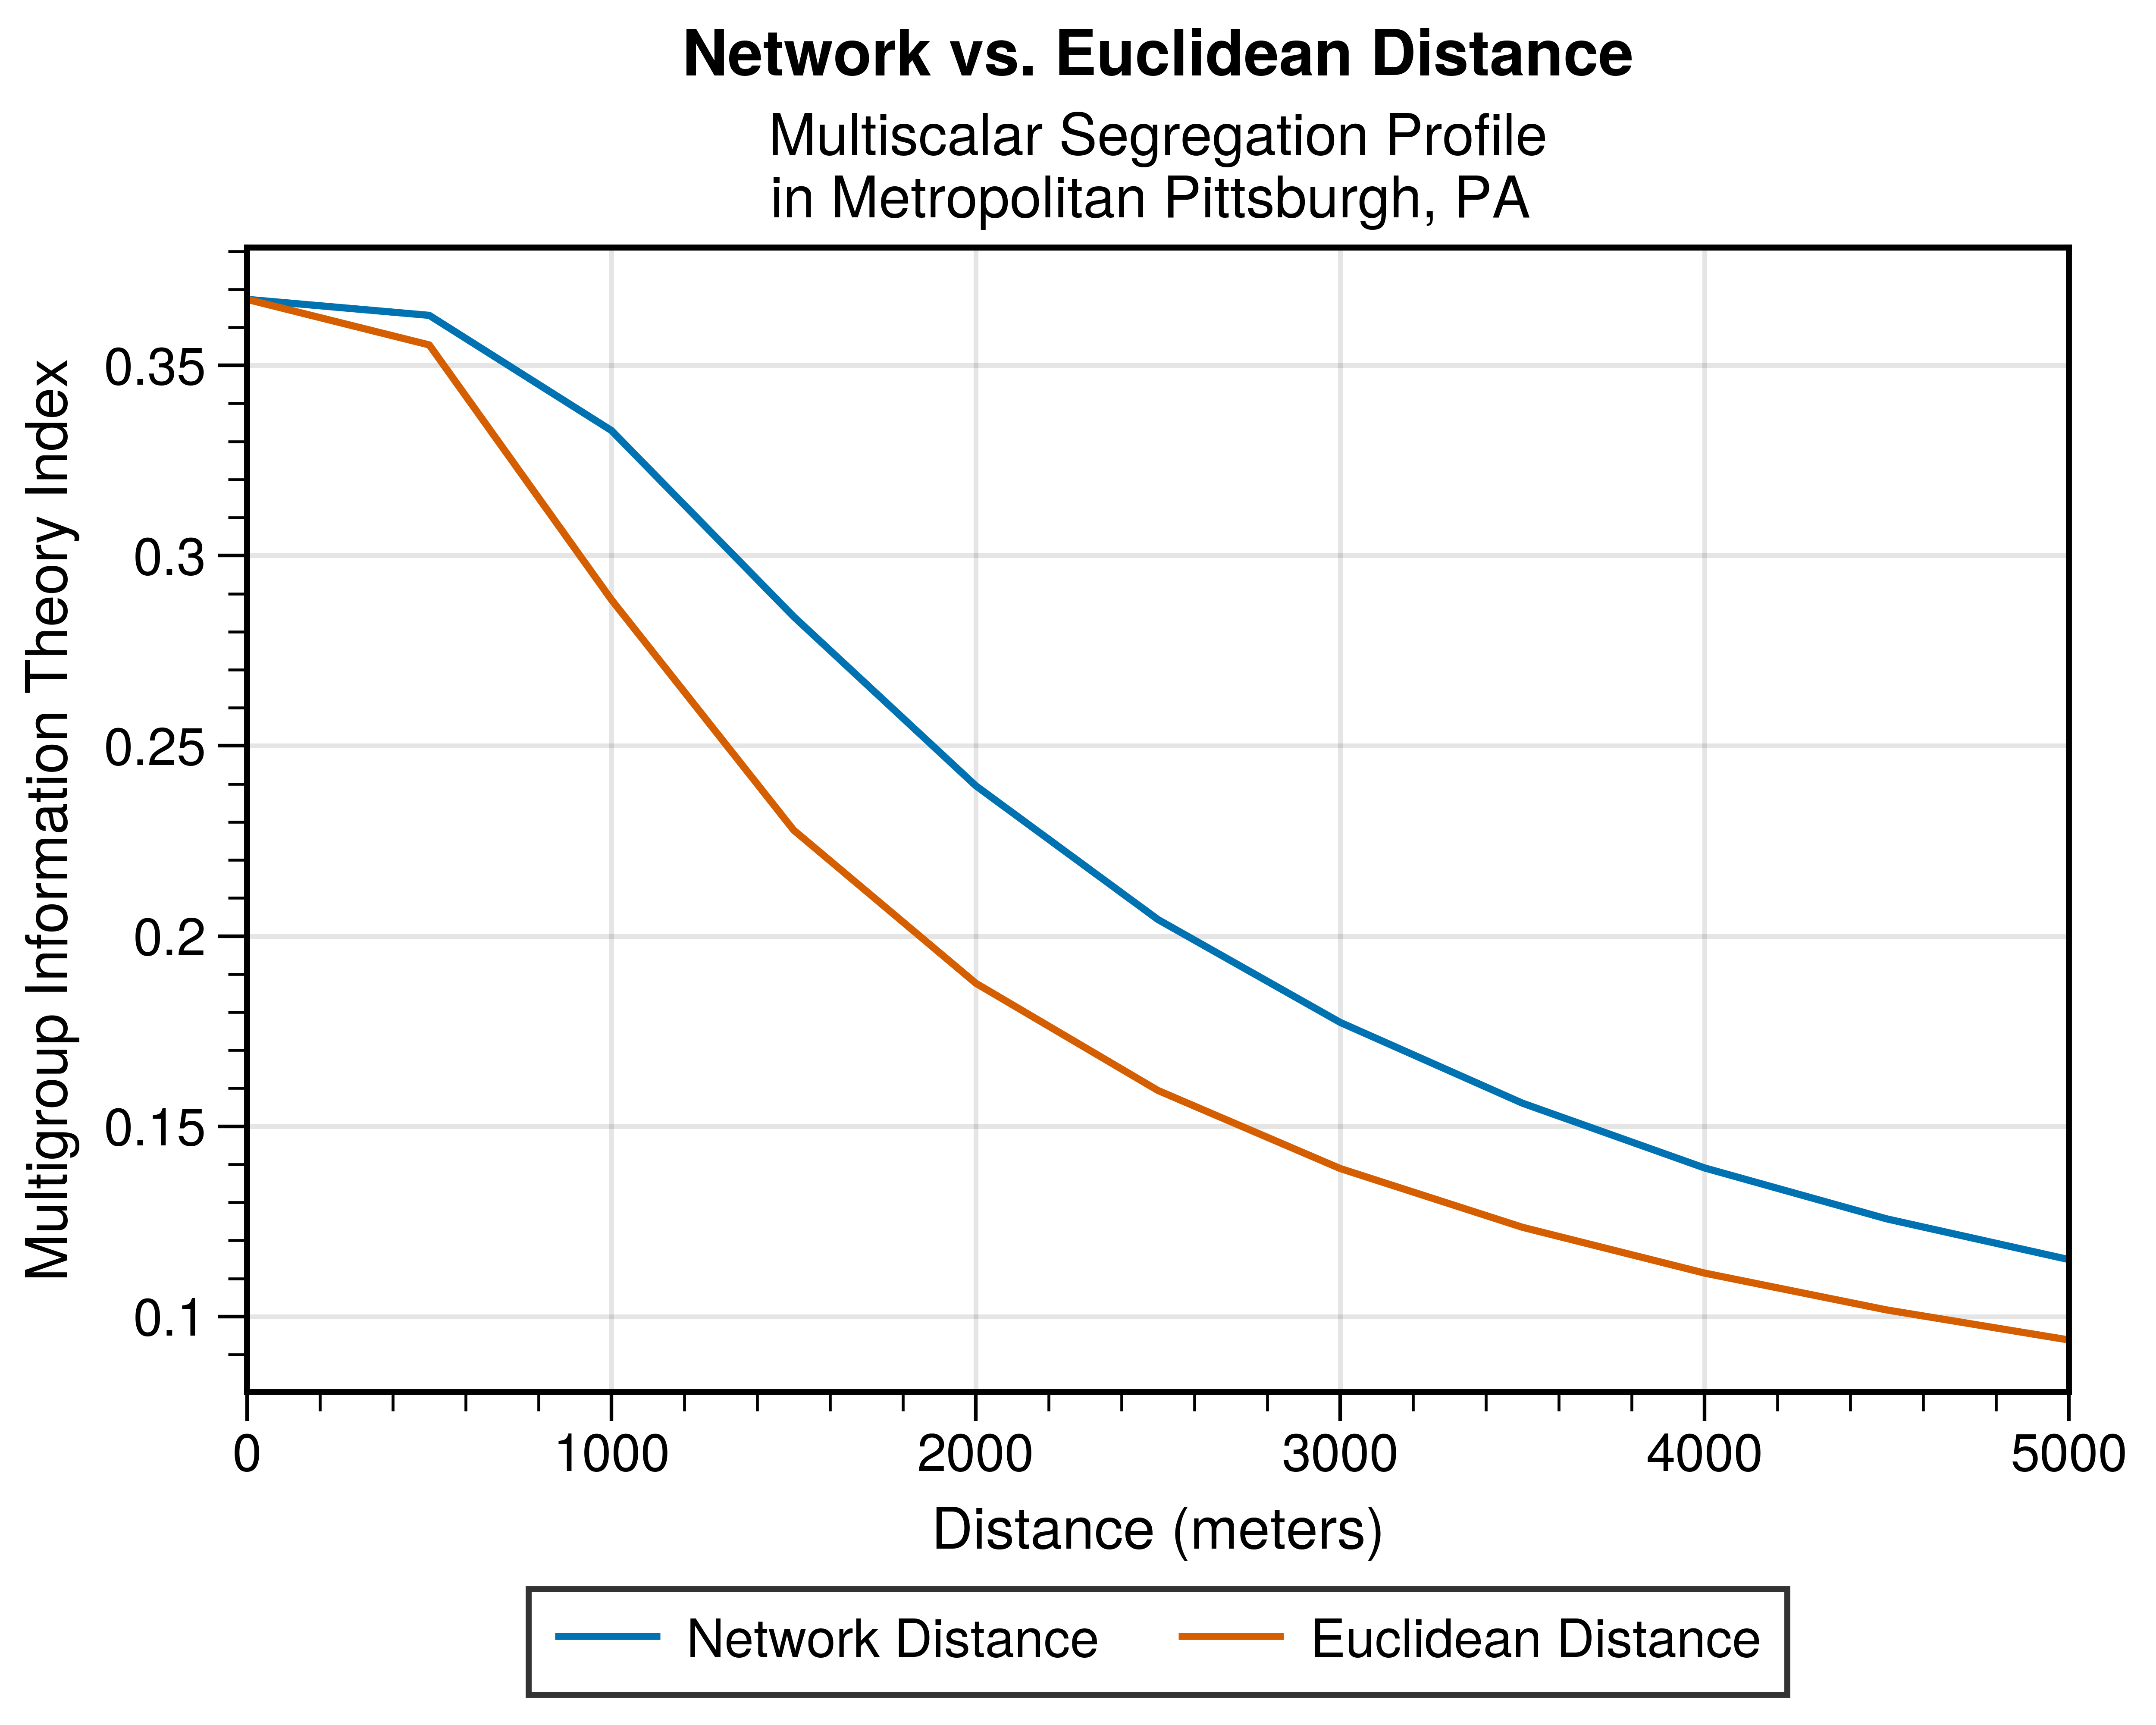
\includegraphics{./pitt_example.png}
\caption{Network vs.~Euclidean Multiscalar Segregation Profiles for
Pittsburgh, PA}\label{fig:multiscalar}
}
\end{figure}

\end{document}
